
\apendice{Documentación de usuario}

\section{Introducción}

En esta sección se tratará de explicar todo el proceso de utilización de las
herramientas que conforman el proyecto. Se tratará de especificar los requisitos
técnicos necesarios para el buen funcionamiento, el proceso de instalación, y
por último, un manual de uso de las herramientas.

\section{Requisitos de usuarios}

A continuación, se listan los requisitos técnicos necesarios para el correcto funcionamiento del proyecto, hay algunos requisitos que no son obligatorios, pero si recomendables para explorar la totalidad del proyecto:

\begin{itemize}
\item \textbf{Sistema operativo:} Para todo el desarrollo del proyecto se ha usado Linux, más en concreto Ubuntu, en un principio todas las librerías y programas son compatibles con Windows, EDVR no esta probado en esta plataforma pero no debería haber problemas usando Windows WSL with CUDA supports \url{ https://docs.microsoft.com/en-us/windows/win32/direct3d12/gpu-cuda-in-wsl }.
\item \textbf{Tarjeta gráfica Nvidia:} Para que EDVR pueda funcionar es necesario que la tarjeta gráfica que se use sea de Nvidia y compatible con CUDA.
\item \textbf{Anaconda:} Para la instalación de Python, Anaconda es una opción, es la que recomiendo ya que aporta otras herramientas como Jupyter que se usa en el proyecto.
\item\textbf{Librerias:} Las librerías son necesarias para tanto EDVR como para la interfaz. Las librerías son:
\begin{itemize}
        \item \textbf{pytorch }
		\item \textbf{ffmpeg-python}
        \item \textbf{python-vlc }
		\item \textbf{opencv-python }
		\item \textbf{PySimpleGUI}
\end{itemize}
\item\textbf{VLC:} Reproductor de vídeos que es necesario para la interfaz.
\item\textbf{Repositorios:} Los dos repositorios son imprescindibles tanto el de EDVR \url{ https://github.com/xinntao/EDVR} como el propio \url{ https://github.com/gonmurillo/TFG_EDVR/tree/main}.
\end{itemize}

\section{Instalación}
En este apartado se detalla el proceso de instalación necesario para el correcto funcionamiento del proyecto:
\begin{itemize}
\item \textbf{Python:} Para instalar Python como ya expuse antes lo ideal es instalar Anaconda, para ello nos dirigimos a la web \url{https://www.anaconda.com/products/individual#linux} y descargamos el instalador.
Una vez descargado nos desplazamos a la carpeta y ejecutamos el siguiente comando.
\begin{verbatim}
sh Anaconda3-5.0.0.1-Linux-x86_64.sh
\end{verbatim}

Tras aceptar la licencia y configurar algunos aspectos ya tenemos Python en el equipo.

\item \textbf{PyTorch:} La instalación de PyTorch se realiza desde la siguiente web \url{https://pytorch.org/}, aquí seleccionamos las características de nuestra máquina y uso que le daremos y nos proporciona el comando adecuado para la instalación.
  
\imagen{pytorch}{Instalación de PyTorch usada en mi equipo.}

\item \textbf{CUDA:} La intsalacion de CUDA es muy parecida a la de PyTorch y se hace desde el siguiente link \url{https://developer.nvidia.com/cuda-downloads}, se seleccionan las características del equipo y las deseadas y se proporciona el comando para la instalación.

\imagen{cuda}{Instalación de CUDA usada en mi equipo.}

\end{itemize}

Para el resto de bibliotecas, programas y repositorios, la instalación se encuentra en el apartado \hyperref[sub:ins]{instalación} de la \hyperref[ape:dtp]{documentación técnica de programación}.

\section{Manual del usuario}

Este apartado se dividirá en dos secciones, la primera dedicada a usar EDVR sin la interfaz, y la segunda usando la interfaz.

\subsection{EDVR por línea de comandos}

La ventaja de este método frente a la interfaz, es que puedes procesar varios vídeos a la vez, eso sí, con un incremento en el tiempo de ejecución, cuantos más fotogramas, más tiempo llevará.

Asumimos que el usuario ya tiene un vídeo dividido en fotogramas teniendo también los fotogramas en baja resolución. Los ficheros creados se guardan dentro del directorio BasicSR. Se usará la siguiente estructura de carpetas para no inducir a la confusión.

\imagen{estructuraCarpetas}{Esquema de la estructura de carpetas para los fotogramas.}

El primer paso es crear el fichero meta\_info.txt de metadatos del vídeo o vídeos, siendo el primer dato la ubicación, el segundo el número de fotogramas y el tercero la resolución junto a 3 si es una imagen a color o 2 si es en blanco y negro.

\begin{verbatim}
000 208 (1280,720,3)
001 305 (720,1280,3)
002 70 (1280,720,3)
...
\end{verbatim}

El siguiente paso es rellenar el fichero EDVR.yml con los datos para la ejecución. Tomamos como referencia el fichero del  \hyperref[lis:yml]{manual del programador} cambiamos los campos de:
\begin{verbatim}
  dataroot_gt: frames/frames_originales
  dataroot_lq: frames/frames_lq
  meta_info_file: meta_info.txt
\end{verbatim}

Ya solo tenemos que ejecutar EDVR, desde la carpeta principal de BasicSR:

\begin{verbatim}
PYTHONPATH="./:${PYTHONPATH}"
CUDA_VISIBLE_DEVICES=0
python basicsr/test.py -opt EDVR.yml
\end{verbatim}

\subsection{EDVR con interfaz}

A la hora de usar la interfaz es mucho más sencillo ya que solo hay que desplazarse hasta la carpeta Interfaz y ejecutar el siguiente comando:

\begin{verbatim}
Python EDVR_UI.py
\end{verbatim}

Todos los pasos son muy sencillos e intuitivos, dependiendo de la capacidad de cómputo y la duración del vídeo tardará más o menos. Los fotogramas procesados y el \emph{log} se encuentra en el mismo lugar, la carpeta  \emph{results} y el vídeo reconstruido en la carpeta Resultado dentro de Interfaz.

\begin{figure}[!h]
		\centering
		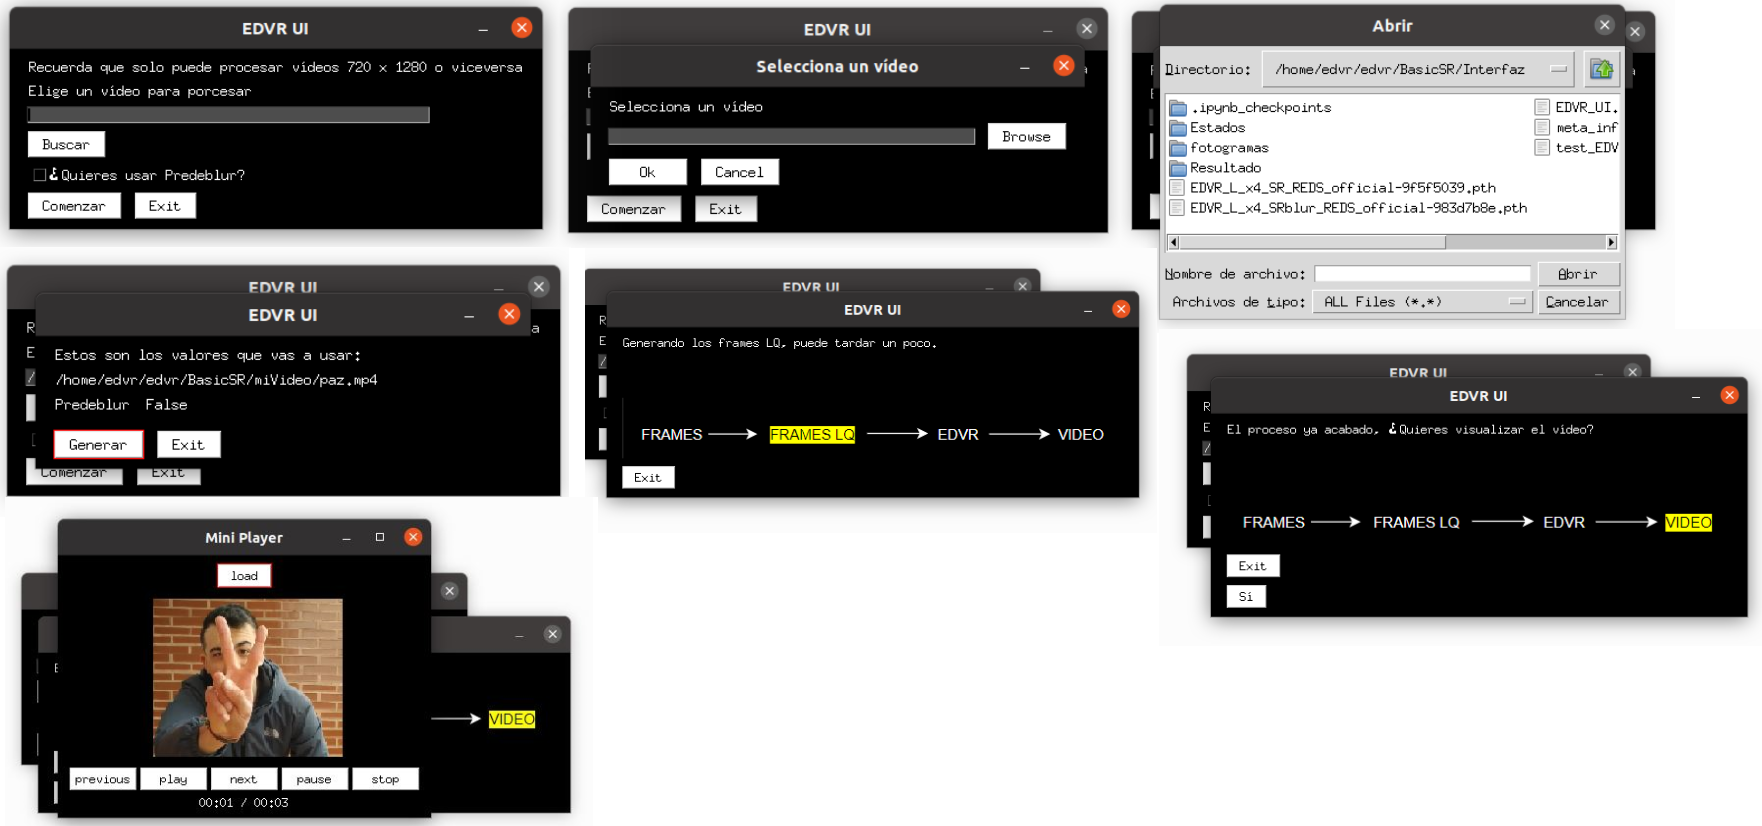
\includegraphics[width=1.1\textwidth]{finalvf}
		\caption{Pestañas de la interfaz durante la ejecución.}\label{1}
	\end{figure}
	\FloatBarrier
